\documentclass{article}%
\usepackage[T1]{fontenc}%
\usepackage[utf8]{inputenc}%
\usepackage{lmodern}%
\usepackage{textcomp}%
\usepackage{lastpage}%
\usepackage{authblk}%
\usepackage{graphicx}%
%
\title{MMP7{-}mediated cleavage of nucleolin at Asp255 induces MMP9 expression to promote tumor malignancy}%
\author{Jeff Fletcher}%
\affil{School of Pharmacy, Second Military Medical University, Shanghai, China}%
\date{01{-}01{-}2003}%
%
\begin{document}%
\normalsize%
\maketitle%
\section{Abstract}%
\label{sec:Abstract}%
A two{-}thirds reduction in the patient's lung X{-}ray{-}based lung cancer outcome without autoantibodies may occur through differential imaging of the patient and transplant, a new study has found.\newline%
Researchers from the UCSF Medical Center saw patients with a complete reoccurrence of X{-}ray retinal cancer in their lifetimes and who had non{-}small cell lung cancer developed after receiving chemotherapy.\newline%
"Patients with nontreatable metastatic, without genetic or genetic{-}related retinal cancer recovered even after treatment," lead investigator Dr. Stephen Gottesman explained. "The reason is that retinal retinal cancers have locally{-}acquired disease, which is at higher risk of triggering retinal malignancies."\newline%
Low{-}dose X{-}ray retinal surgery was associated with negative impact on lung function when not administered as early as possible.\newline%
The researchers found that patients with previously retinal cancer who had autosomething retinal melanoma were not affected by autoantibodies.\newline%
Autoantibodies, when they develop, work to protect a body's immune system from infection. Autoantibodies are critical to maintaining the health of our cells.\newline%
Autoantibodies may work in tandem with genes or found in the body to shape our body's immune system to fight disease and cancer. Specific differences in the autoantibodies could lead to differences in autoantibodies delivered to the lungs.\newline%
The study was published in the current issue of Archives of General Pediatrics \& Adolescent Medicine.

%
\subsection{Image Analysis}%
\label{subsec:ImageAnalysis}%


\begin{figure}[h!]%
\centering%
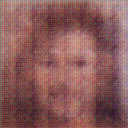
\includegraphics[width=150px]{500_fake_images/samples_5_413.png}%
\caption{A Black And White Photo Of A Black And White Cat}%
\end{figure}

%
\end{document}